%----------------------------------------------------------------------------------------
%	CHAPTER 2
%----------------------------------------------------------------------------------------
\chapterimage{ChapterImages/chapter2.png} % Chapter heading image

\chapter{Linux File System, Command Line Interface, Users, and Groups}
\label{ch:users-groups}

\section{Introduction to the Linux File System}

The Linux file system is the foundation of how your computer organizes and stores data.
Think of it like a well-organized library where every book (file) has its specific place on a shelf (directory).
Understanding how this system works is essential for anyone working with Linux, since almost every task in this course — from running programs to configuring services — ultimately comes down to reading, writing, or navigating files.

\textbf{Key Concepts:}
\begin{itemize}
    \item \textbf{Efficient Organization:} The Linux file system arranges data in a logical, hierarchical structure. Everything has a place and a purpose, making it easy to find and manage files.
    \item \textbf{System Navigation:} Just like learning to navigate a new building, understanding the file system helps you move around your computer efficiently. You will learn where programs are stored, where your personal files live, and where system configurations are kept.
    \item \textbf{Command Line Interface (CLI):} The CLI is your direct line of communication with the file system. While graphical interfaces are user-friendly, the command line gives you powerful tools to interact with files and directories quickly and precisely.
\end{itemize}

The file system is not just about storage — it is about control. It manages \textbf{permissions} (who can access what), \textbf{tracks changes}, and \textbf{ensures data integrity}.
As you progress through this chapter, you will see that the file system is the backbone of everything that happens on a Linux machine.

\subsection{What is a File System?}
A file system is like the organizational system in a filing cabinet. Just as you need a method to organize paper documents, your computer needs a system to organize digital files on disk.

\textbf{Core Functions:}
\begin{itemize}
    \item \textbf{Storage Control:} The file system decides exactly how data is written to your hard drive and how it is retrieved. When you save a file, the file system determines where on the disk it goes; when you open a file, it knows exactly where to find it.
    \item \textbf{Organization:} Files are grouped into directories (folders), which can contain other directories, creating a tree-like structure. This hierarchy keeps everything organized and accessible.
    \item \textbf{Access Management:} The file system controls permissions — who can read, write, or execute files. This security layer protects sensitive data and prevents unauthorized access. We cover this in detail in Chapter~\ref{ch:permissions}.
    \item \textbf{Metadata Management:} Beyond just storing your data, the file system tracks metadata such as file size, creation date, modification date, and ownership.
\end{itemize}

\section{Common Linux File Systems}
Linux supports several file systems, each with different strengths. The three most common are \textbf{ext4}, \textbf{XFS}, and \textbf{Btrfs}.

\subsection{ext4 (Fourth Extended Filesystem)}
A stable and widely used file system, ideal for general-purpose Linux installations.
\begin{itemize}
    \item Default on most Linux distributions; highly reliable and well-tested
    \item Large file and volume support (files up to 16\,TiB, volumes up to 1\,EiB)
    \item Journaling ensures quick recovery after crashes
    \item Efficient performance through extents and delayed allocation
    \item Backward compatible with ext2/ext3
\end{itemize}
\textbf{Best for:} Desktops, laptops, and general-purpose servers.

\subsection{XFS}
A high-performance file system designed for handling large files efficiently.
\begin{itemize}
    \item Excellent scalability for very large storage volumes
    \item Optimized for parallel I/O and high-speed data access
    \item Journaling for quick crash recovery
    \item Fast metadata operations and file system repair (via \texttt{xfs\_repair})
    \item Ideal for heavy workloads such as video editing or databases
\end{itemize}
\textbf{Best for:} High-performance systems and large data workloads.

\subsection{Btrfs (B-tree Filesystem)}
A modern, feature-rich file system built for flexibility, data protection, and advanced management.
\begin{itemize}
    \item Built-in RAID support and disk pooling
    \item Snapshots and subvolumes for easy backups and rollbacks
    \item Data integrity checks using checksums
    \item Online resizing and defragmentation
    \item Support for transparent compression and deduplication
\end{itemize}
\textbf{Best for:} Systems requiring advanced storage features and data reliability.

\subsubsection*{Comparison Summary}
\begin{table}[h!]
\centering
\small
\renewcommand{\arraystretch}{1.3}
\begin{tabular}{|>{\centering\arraybackslash}p{4cm}|>{\centering\arraybackslash}p{3cm}|>{\centering\arraybackslash}p{3cm}|>{\centering\arraybackslash}p{3cm}|}
\hline
\textbf{Feature} & \textbf{ext4} & \textbf{XFS} & \textbf{Btrfs} \\ \hline
Journaling & Yes & Yes & Yes \\ \hline
Snapshots / RAID & No & No & Yes \\ \hline
Performance & Balanced & Excellent for large files & Moderate \\ \hline
Scalability & High & Very High & High \\ \hline
Max File Size & Up to 16 TiB & Up to 8 EiB & Up to 16 EiB \\ \hline
Max Volume Size & Up to 1 EiB & Up to 8 EiB & Up to 16 EiB \\ \hline
Best Use Case & General-purpose systems & Large-file and high-performance workloads & Advanced storage and data integrity \\ \hline
\end{tabular}
\caption{Comparison of Common Linux File Systems}
\label{tab:filesystem-comparison}
\end{table}

\noindent\textbf{Checking the file system of a mounted volume:}
\begin{lstlisting}[language=Terminal]
$ df -Th
\end{lstlisting}
The \texttt{-T} flag adds a column showing the file system type (ext4, xfs, btrfs, \dots) for each mounted volume, and \texttt{-h} prints sizes in a human-readable form (GB, TB, \dots).

\section{The Linux File System Hierarchy}
Linux organizes everything into a single tree structure, starting from the \texttt{root} directory (\texttt{/}). Every file, folder, and device stems from this root, forming a unified hierarchy — unlike Windows, there is no separate \texttt{C:}, \texttt{D:}, etc.\ drive letter; every storage device is \emph{mounted} somewhere inside this same tree.

\textbf{Root Directory (\texttt{/}):} The starting point of the entire file system. All other directories branch from here.

\textbf{\texttt{/home} -- User Home Directories:}
Stores personal files and user-specific configuration. Each user has a separate folder under \texttt{/home}.
\begin{itemize}
    \item Contains documents, downloads, and hidden configuration files (\texttt{.bashrc}, \texttt{.config/})
    \item Each user has a private workspace, e.g.\ \texttt{/home/student/}
    \item Comparable to ``My Documents'' on Windows
\end{itemize}

\textbf{\texttt{/etc} -- System Configuration Files:}
Holds system-wide configuration and initialization files used by Linux and applications.
\begin{itemize}
    \item Includes user and network settings (\texttt{/etc/passwd}, \texttt{/etc/network/})
    \item Files are plain text and editable, but usually require root privileges to modify
    \item Always back up a configuration file before editing it
\end{itemize}

\textbf{\texttt{/var} -- Variable Data Files:}
Contains files that change frequently during system operation.
\begin{itemize}
    \item Logs (\texttt{/var/log/}), caches (\texttt{/var/cache/}), and spools (\texttt{/var/spool/})
    \item Grows over time; disk usage here should be monitored
    \item Useful for troubleshooting system behavior
\end{itemize}

\textbf{\texttt{/tmp} -- Temporary Files:}
Used for temporary data created by programs or users.
\begin{itemize}
    \item Cleared automatically on reboot (on most distributions)
    \item Accessible to all users
    \item Not suitable for storing important data
\end{itemize}

\textbf{\texttt{/dev} -- Device Files:}
Represents hardware devices as special files that applications can access.
\begin{itemize}
    \item \texttt{/dev/sda} $\rightarrow$ first hard drive, \texttt{/dev/sda1} $\rightarrow$ its first partition
    \item \texttt{/dev/null} $\rightarrow$ discards all data written to it
    \item Managed automatically by the system (via \texttt{udev})
    \item Enables programs to interact with hardware through ordinary file operations
\end{itemize}

\subsection{Other Important Directories}
\textbf{\texttt{/bin} -- Essential User Commands:} Core command-line utilities needed for basic system operation (e.g.\ \texttt{ls}, \texttt{cp}, \texttt{mv}, \texttt{mkdir}).

\textbf{\texttt{/sbin} -- System Administration Commands:} System management tools for administrators (e.g.\ \texttt{reboot}, \texttt{shutdown}, \texttt{fdisk}).

\textbf{\texttt{/usr} -- User Applications and Libraries:} Stores most user-installed software and shared resources.
\begin{itemize}
    \item \texttt{/usr/bin/} $\rightarrow$ common programs
    \item \texttt{/usr/lib/} $\rightarrow$ libraries
    \item \texttt{/usr/share/} $\rightarrow$ documentation, icons, and other shared data
\end{itemize}

\textbf{\texttt{/boot} -- Boot Files:} Contains the Linux kernel and boot loader configuration files needed to start the system.

\textbf{\texttt{/opt} -- Optional Software:} Used for manually installed or third-party applications (e.g.\ Google Chrome, VirtualBox).

\subsection{Visual Overview}
Figure~\ref{fig:fs-hierarchy} summarizes the directories introduced above as branches of the same root tree. Note that this is a small, teaching-oriented subset — a real system also has directories such as \texttt{/proc}, \texttt{/sys}, \texttt{/lib}, \texttt{/mnt}, and \texttt{/root} (the home directory of the root user, not to be confused with \texttt{/}).

\begin{figure}[h]
    \centering
    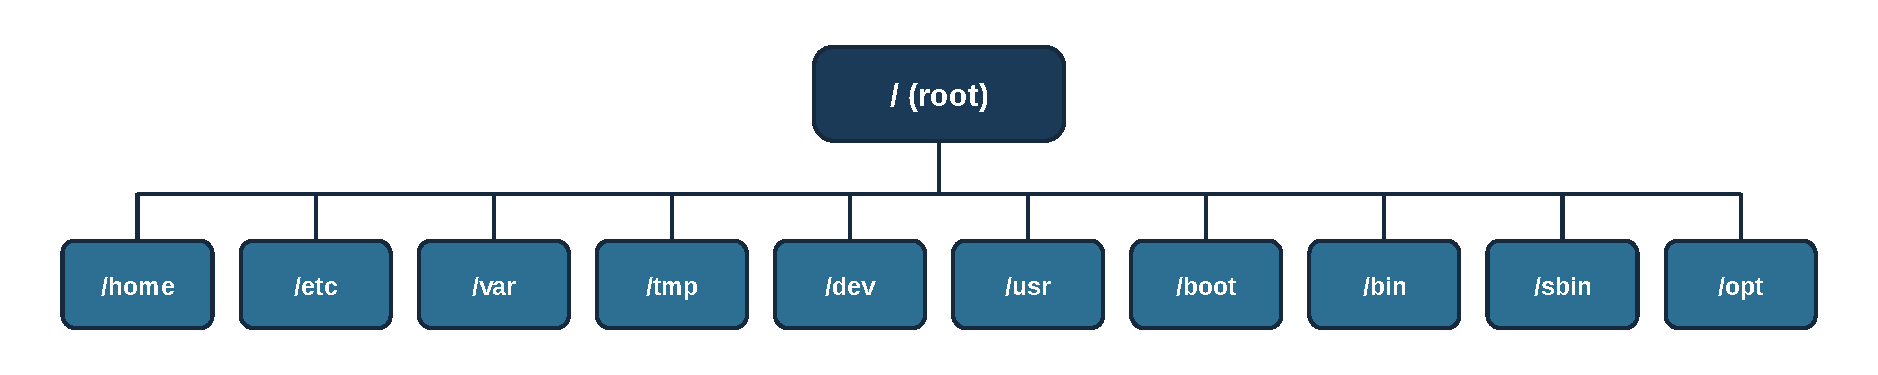
\includegraphics[width=0.95\textwidth]{Images/Chapter2/fs-hierarchy-tree.pdf}
    \caption{The Linux file system hierarchy: every directory branches from the single root (\texttt{/}).}
    \label{fig:fs-hierarchy}
\end{figure}

\section{The Command Line Interface (CLI)}
The CLI allows you to interact with Linux by typing commands instead of clicking through a graphical interface. It is more \textbf{powerful}, \textbf{precise}, \textbf{fast}, and \textbf{consistent} once you get used to it, and it is the primary way you will interact with Linux throughout this course.

\textbf{What is the CLI?}
\begin{itemize}
    \item A text-based interface for entering commands.
    \item Think of it as telling the computer exactly what to do, instead of pointing at icons.
\end{itemize}

\textbf{Why Use the CLI?}
\begin{itemize}
    \item \textbf{Powerful:} Work with multiple files, chain commands, automate tasks, and access features not exposed in any GUI.
    \item \textbf{Precise:} Commands do exactly what you type, with no ambiguity.
    \item \textbf{Fast:} Once learned, typing commands is quicker than navigating menus.
    \item \textbf{Portable:} Works on servers, remote systems, and across Linux distributions, even without a graphical environment installed.
\end{itemize}

\subsection{Terminal Emulators}
A \textbf{terminal emulator} is the application window in which you type commands; the CLI itself is provided underneath by the \textbf{shell} (commonly \texttt{bash}). Common terminal emulators include:
\begin{itemize}
    \item \textbf{GNOME Terminal:} default on Ubuntu/GNOME
    \item \textbf{Konsole:} default on KDE
    \item \textbf{xterm:} lightweight, classic terminal
    \item \textbf{Terminator:} supports split-screen layouts
    \item \textbf{Tilix:} tiling terminal emulator
\end{itemize}

\subsection{Understanding the Prompt}
When you open a terminal, you usually see something like:
\begin{lstlisting}[language=Terminal]
student@linux:~$
\end{lstlisting}
Each part tells you important information about your session, and the command you type generally follows the same predictable pattern of \texttt{command}, \texttt{options}, and \texttt{arguments}. Figure~\ref{fig:command-anatomy} breaks both down visually.

\begin{enumerate}
    \item \textbf{\texttt{student} -- Username:} the account currently logged in.
    \item \textbf{\texttt{@} -- Separator:} separates the username from the computer name.
    \item \textbf{\texttt{linux} -- Hostname:} identifies the machine you are working on; useful when managing multiple computers or connecting remotely over SSH.
    \item \textbf{\texttt{:} -- Separator:} separates the host information from the current working directory.
    \item \textbf{\texttt{\textasciitilde} -- Current Directory:} shows the directory you are currently in (\texttt{\textasciitilde} is shorthand for your home directory).
    \item \textbf{\texttt{\$} -- Prompt Symbol:} indicates the type of user:
    \begin{itemize}
        \item \texttt{\$} $\rightarrow$ regular user
        \item \texttt{\#} $\rightarrow$ root (administrator)
    \end{itemize}
\end{enumerate}

\begin{figure}[h]
    \centering
    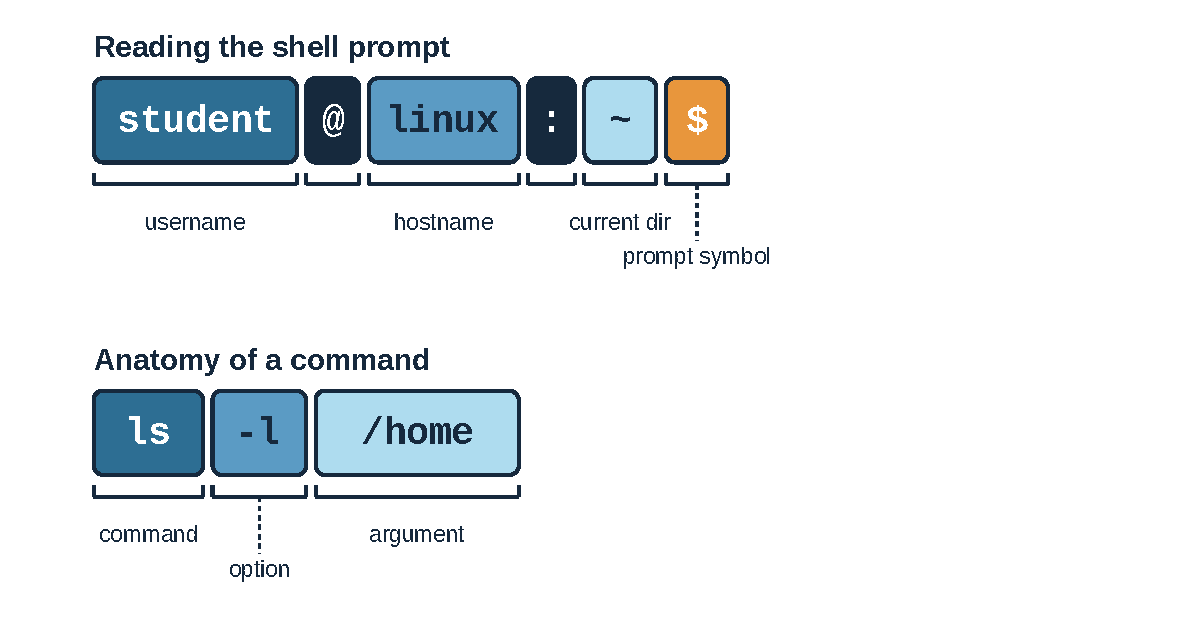
\includegraphics[width=0.8\textwidth]{Images/Chapter2/command-anatomy.pdf}
    \caption{Reading the shell prompt, and the general anatomy of a command.}
    \label{fig:command-anatomy}
\end{figure}

\subsubsection{Basic Terminal Usage}
Steps to run a command:
\begin{enumerate}
    \item Type a command at the prompt.
    \item Press \texttt{Enter} to execute it.
    \item View the output.
    \item Receive a new prompt for the next command.
\end{enumerate}

\textbf{Command Structure:}
\begin{lstlisting}[language=Terminal]
command [options] [arguments]
\end{lstlisting}
\begin{itemize}
    \item \texttt{command}: the action you want to perform
    \item \texttt{options} (or \emph{flags}): modify how the command behaves (optional)
    \item \texttt{arguments}: the files, directories, or targets the command acts on (optional)
\end{itemize}

\textbf{Example:}
\begin{lstlisting}[language=Terminal]
$ ls -l /home
\end{lstlisting}
\begin{itemize}
    \item \texttt{ls} $\rightarrow$ list directory contents
    \item \texttt{-l} $\rightarrow$ long format (detailed info)
    \item \texttt{/home} $\rightarrow$ directory to list
\end{itemize}

\textbf{Getting Help:} Almost every command documents itself. Before guessing what a flag does, check:
\begin{lstlisting}[language=Terminal]
$ man ls           # full manual page (press q to quit)
$ ls --help        # short usage summary
\end{lstlisting}

\subsubsection{Navigation Commands}

\textbf{\texttt{pwd} -- Print Working Directory:} shows your current directory.
\begin{lstlisting}[language=Terminal]
$ pwd
/home/student
\end{lstlisting}

\textbf{\texttt{ls} -- List Directory Contents:} shows files and directories in the current location.
\begin{lstlisting}[language=Terminal]
$ ls
Documents  Downloads  Pictures
\end{lstlisting}
\textbf{Common options:}
\begin{itemize}
    \item \texttt{ls -l} $\rightarrow$ detailed (long) list
    \item \texttt{ls -a} $\rightarrow$ include hidden files (names starting with \texttt{.})
    \item \texttt{ls -lh} $\rightarrow$ long list with human-readable sizes
\end{itemize}
\textbf{Tip:} Options can be combined: \texttt{ls -lah} $\rightarrow$ long, all files, human-readable sizes.

\textbf{\texttt{cd} -- Change Directory:} moves between directories.
\begin{lstlisting}[language=Terminal]
$ cd Documents       # go into Documents
$ cd ..              # go up one level (parent directory)
$ cd /               # go to the root directory
$ cd ~               # go to the home directory
$ cd -               # go to the previous directory
\end{lstlisting}
\textbf{Absolute path:} starts from the root (\texttt{/}), e.g.\ \texttt{/home/student/Documents}.\\
\textbf{Relative path:} starts from the current directory, e.g.\ \texttt{Documents/report.txt}.

\subsection{File and Directory Operations}

\textbf{\texttt{mkdir} -- Create Directories:}
\begin{lstlisting}[language=Terminal]
$ mkdir project              # create a single directory
$ mkdir -p project/src/lib   # create nested directories in one step
\end{lstlisting}
\textbf{Tip:} A directory name containing spaces (e.g.\ \texttt{lab practice}) must be quoted or escaped, e.g.\ \texttt{mkdir "lab practice"} or \texttt{mkdir lab\textbackslash{} practice} -- otherwise the shell treats it as two separate arguments.

\textbf{\texttt{rmdir} -- Remove Empty Directories:}
\begin{lstlisting}[language=Terminal]
$ rmdir empty_folder
\end{lstlisting}
\texttt{rmdir} only works on empty directories; to remove a directory and everything inside it, use \texttt{rm -r} (below).

\textbf{\texttt{touch} -- Create a File:} creates an empty file, or updates its timestamp if it already exists.
\begin{lstlisting}[language=Terminal]
$ touch newfile.txt
$ touch file1.txt file2.txt file3.txt
\end{lstlisting}

\textbf{\texttt{cp} -- Copy Files/Directories:}
\begin{lstlisting}[language=Terminal]
$ cp file.txt /home/student/Documents/       # copy a file
$ cp -r folder1/ folder2/                    # copy a folder recursively
$ cp -p file.txt backup.txt                  # preserve permissions and timestamps
$ cp -i file.txt existing.txt                # ask before overwriting
\end{lstlisting}
\textbf{Tip:} Use the wildcard \texttt{*} to match multiple files, e.g.\ \texttt{cp *.txt /backup/} copies every \texttt{.txt} file in the current directory.

\textbf{\texttt{mv} -- Move/Rename Files:}
\begin{lstlisting}[language=Terminal]
$ mv oldname.txt newname.txt                 # rename a file
$ mv file.txt /home/student/Documents/       # move a file
$ mv folder1/ /new/location/                 # move a folder
$ mv -i file.txt existing.txt                # ask before overwriting
\end{lstlisting}
\textbf{Note:} Unlike \texttt{cp}, \texttt{mv} does not leave a copy behind — the original is removed from the source location.

\textbf{\texttt{rm} -- Remove Files/Directories (permanent!):}
\begin{lstlisting}[language=Terminal]
$ rm file.txt                # delete a file
$ rm -r folder/              # delete a directory recursively
$ rm -f file.txt             # force delete, no confirmation
$ rm -rf folder/             # force recursive delete
\end{lstlisting}

\faExclamationTriangle\ \textbf{DANGER ZONE:}
\begin{lstlisting}[language=Terminal]
$ rm -rf /
\end{lstlisting}
\textbf{Never run this.} It recursively force-deletes every file the current user can reach, starting from the root directory. Modern versions of \texttt{rm} refuse to run this exact command on \texttt{/} without an extra flag, but close variants (e.g.\ with a typo'd path, or run as root) can still destroy a system with no way to undo it. There is no ``Recycle Bin'' on the command line: \texttt{rm} deletes immediately and permanently.

\subsection{Combining Commands}
The shell lets you combine simple commands into more powerful ones:
\begin{itemize}
    \item \texttt{cmd1 ; cmd2} -- run \texttt{cmd1}, then \texttt{cmd2}, regardless of whether \texttt{cmd1} succeeded.
    \item \texttt{cmd1 \&\& cmd2} -- run \texttt{cmd2} only if \texttt{cmd1} succeeded.
    \item \texttt{cmd1 | cmd2} -- a \textbf{pipe}: send the output of \texttt{cmd1} directly into \texttt{cmd2} as its input.
    \item \texttt{cmd > file} -- redirect a command's output into \texttt{file}, overwriting it.
    \item \texttt{cmd >> file} -- redirect a command's output into \texttt{file}, appending to it.
\end{itemize}
\begin{lstlisting}[language=Terminal]
$ mkdir logs && cd logs        # only enter logs/ if it was created successfully
$ ls -l | grep ".txt"          # list files, then filter for ones containing ".txt"
$ echo "done" >> status.log    # append a line to a log file
\end{lstlisting}

\textbf{Lab Tips:}
\begin{itemize}
    \item Always check the prompt before running a command. It shows who you are and where you are, which helps prevent mistakes, especially with \texttt{rm}, \texttt{mv}, or other destructive commands.
    \item When connected to a remote machine via SSH, the hostname part of the prompt is especially helpful to avoid running a command on the wrong machine.
    \item Use \texttt{Tab} completion to save typing and avoid typos in file names.
    \item Use the \texttt{Up} arrow (or \texttt{history}) to reuse previous commands instead of retyping them.
\end{itemize}

\section{Users}
Users are the entities that log into the system or own running processes — in other words, everything that happens on Linux happens \emph{as} some user. Each user is identified by a unique numerical \textbf{User ID (UID)}.

\begin{enumerate}
    \item \textbf{Root User:} The root user has the highest level of access and can read or modify any file, use any command, and control any system resource. The root user's UID is always \textbf{0}.
    \item \textbf{Regular Users:} Regular users have limited access to files and resources. They cannot perform sensitive operations, such as installing or modifying system-level software, without explicit permission. On most modern distributions, regular user UIDs start at \textbf{1000}.
    \item \textbf{System Users:} System users are created to run services and background processes, such as database servers. They usually cannot log in interactively and have access only to the resources their specific service needs. System user UIDs are typically in the range \textbf{1--999}.
\end{enumerate}

\subsection{The \texttt{sudo} Command}
When Linux is installed, the first user is created as a regular user, and direct login to the root account is usually disabled entirely. Users allowed to run \texttt{sudo} are listed in the \textbf{sudoers} file (\texttt{/etc/sudoers}); the first user created during installation is normally added there automatically.

Using \texttt{sudo}, an authorized user can temporarily act as root (\texttt{UID~=~0}) and gain full system access for a single command:
\begin{lstlisting}[language=Terminal]
$ sudo <intended command>
\end{lstlisting}

\subsubsection*{Security Note}
When you run \texttt{sudo}, the system asks for \textbf{your own password}, not the root password. If your account is not listed in \texttt{/etc/sudoers}, the command fails with:
\begin{center}
    \texttt{user is not in the sudoers file. This incident will be reported.}
\end{center}

\subsection{The \texttt{/etc/passwd} and \texttt{/etc/shadow} Files}
\textbf{\texttt{/etc/passwd}:} contains basic account information such as username, UID, home directory, and default shell. It is readable by all users.

\textbf{\texttt{/etc/shadow}:} contains encrypted passwords, along with password expiration and account restriction data. It can only be read by the root user or specific privileged system programs.

\subsection{User Management Commands}
\begin{enumerate}
    \item \textbf{\texttt{useradd}:} adds a new user.
\begin{lstlisting}[language=Terminal]
$ sudo useradd username
$ sudo useradd -m -s /bin/bash username
\end{lstlisting}
    \texttt{-m}: creates a home directory for the new user.\\
    \texttt{-s}: sets the user's default shell.

    \item \textbf{\texttt{passwd}:} sets or changes a user's password.
\begin{lstlisting}[language=Terminal]
$ sudo passwd username
\end{lstlisting}

    \item \textbf{\texttt{userdel}:} deletes a user.
\begin{lstlisting}[language=Terminal]
$ sudo userdel username
$ sudo userdel -r username   # also delete the user's home directory
\end{lstlisting}
\end{enumerate}

\section{Groups}
Groups are collections of users who share access to system resources. Each group is identified by a unique numerical \textbf{Group ID (GID)}.

\begin{enumerate}
    \item \textbf{Primary Group:} every user has one primary group, recorded in \texttt{/etc/passwd}. On many distributions, creating a new user automatically creates a new group with the same name and makes the user its only member — the \textbf{User Private Group} policy, which simplifies access management.
    \item \textbf{Secondary Groups:} a user can additionally belong to any number of secondary groups, which grant extra permissions for shared resources. For example, everyone on a project team can be added to a shared \texttt{project} group so that they can all read, modify, or write the project's files.
\end{enumerate}

\subsection{Group Management Commands}
\begin{enumerate}
    \item \textbf{\texttt{groupadd}:} adds a new group.
\begin{lstlisting}[language=Terminal]
$ sudo groupadd groupname
\end{lstlisting}
    \item \textbf{\texttt{groupdel}:} deletes a group.
\begin{lstlisting}[language=Terminal]
$ sudo groupdel groupname
\end{lstlisting}
    \item \textbf{\texttt{gpasswd}:} adds or removes a user from a group.
\begin{lstlisting}[language=Terminal]
$ sudo gpasswd -a username groupname   # add
$ sudo gpasswd -d username groupname   # remove
\end{lstlisting}
    \item \textbf{\texttt{getent}:} looks up the members of a group.
\begin{lstlisting}[language=Terminal]
$ getent group groupname
\end{lstlisting}
    \textbf{Tip:} \texttt{groups username} and \texttt{id username} are quick ways to see which groups a user currently belongs to.
\end{enumerate}

\section{Hands-on Practices}
Bellow you see a list of tasks. Complete the tasks using the Linux terminal and record the commands you use. Where requested, explain the results of your commands.

\subsection{Exercise 1: Build and manage a project directory}
Create the following directory structure inside your home directory:

\begin{lstlisting}[language=bash]
os-lab/
|-- documents/
| |-- report.txt
|  -- notes.txt
|-- scripts/
 -- backup/
\end{lstlisting}

Complete the following tasks:
\begin{enumerate}
	\item Create the directory structure, including all required subdirectories.
	\item Create report.txt, notes.txt, and file named todo.txt inside scripts/.
	\item Rename notes.txt to meeting-notes.txt.
	\item Copy report.txt into backup/.
	\item Move todo.txt from scripts/ to documents/.
	\item Create an empty directory named empty-dir/ and remove it.
	\item Display the final directory tree or an equivalent recursive listing to verify your work.
\end{enumerate}

Now, answer the following questions:
\begin{itemize}
	\item What is the difference between copying and moving a file? \item Why does \texttt{rmdir} fail when a directory is not empty? \item What happens if you copy a file to a destination where a file with the same name already exists?
\end{itemize}

\subsection{Exercise 2: Investigate File Information and Hidden Files}
Perform the following tasks inside your \texttt{os-lab/} directory:
\begin{enumerate}
	\item Create three text files named \texttt{data1.txt}, \texttt{data2.txt}, and \texttt{data3.txt}, and one file named \texttt{README}.
	\item Add different lines of text to the three \texttt{.txt} files. Ensure that the files contain different numbers of lines.
	\item Create a hidden file named \texttt{.lab-config}. \item List the directory contents normally and then list them again, including hidden files.
	\item Display a detailed listing containing file permissions, ownership, file sizes, and modification times.
	\item Copy all \texttt{.txt} files into the \texttt{backup/} directory using a wildcard.
	\item Display the number of lines in each \texttt{.txt} file and identify which file contains the most lines. \end{enumerate}
	
Now, answer the following questions:
\begin{itemize}
	\item Why is \texttt{.lab-config} not displayed by a normal directory listing?
	\item What information can you obtain from a long-format directory listing?
	\item How does the shell expand \texttt{*.txt} before executing a command?
\end{itemize}

\subsection{Exercise 3: Create and Manage Users and Groups}

Create two temporary users named \texttt{Amir} and \texttt{Reza}, each with a home directory and Bash as the login shell. Then complete the following tasks:
\begin{enumerate}
	\item Create a group named \texttt{osproject}.
	\item Add both users to \texttt{osproject} as supplementary-group members.
	\item Verify that both users exist. Inspect their UIDs, primary GIDs, home directories, and supplementary groups.
	\item Set passwords for the accounts if required by your instructor.
	\item Remove \texttt{Reza} from \texttt{osproject} and verify the change.
	\item Restore \texttt{Reza}'s membership in \texttt{osproject} if necessary for Exercise~4.
	\item At the end of the lab, remove the temporary users and group after verifying that you are deleting only the accounts and group created for this exercise.
\end{enumerate}
Now, answer the following questions:
\begin{itemize}
	\item What is the difference between \texttt{useradd} and \texttt{groupadd}?
	\item Why might a user need to log out and log back in before newly assigned supplementary-group membership is reflected in an existing session?
	\item What is the difference between deleting a user and deleting a user together with their home directory?
\end{itemize}

\subsection{Exercise 4: Set Up a Shared Project Directory}
Assume that \texttt{Amir} and \texttt{Reza} are members of the supplementary group \texttt{osproject}. \begin{enumerate}
	\item Create a shared directory named \texttt{/srv/osproject}.
	\item Set its group ownership to \texttt{osproject}.
	\item Configure its permissions so that the owner and group can access the directory, while other users have no access.
	\item Configure the directory so that new files and subdirectories inherit the \texttt{osproject} group.
	\item As \texttt{Amir}, create a file named \texttt{shared.txt} in the directory and add some text to it.
	\item As \texttt{Reza}, verify that you can read and modify \texttt{shared.txt}.
	\item As \texttt{Reza}, create a second file in the shared directory.
	\item Inspect the ownership and permissions of the directory and both files. Explain any differences you observe.
	\item Attempt to access the directory as an unrelated ordinary user, if one is available in the lab, and verify that access is denied.
	\item Explain how you would modify the configuration if project members should be able to read and modify project files while unrelated users should retain read-only access.
\end{enumerate}
Now, answer the following questions:
\begin{itemize}
	\item What is the difference between file ownership and group ownership?
	\item Why might group write permission on a directory be necessary even if users can write to an existing file?
	\item Does setting the setgid bit on a directory automatically make every new file group-writable?
\end{itemize}